Sběrnice MTBbus vznikla v roce 2000 \cite{mtb:web}, kdy se hledal vhodný systém
pro programovatelné počítačové řízení modelové železnice v Klubu modelářů
železnic Brno I (\gls{kmz}), jehož je autor této práce členem.
\textit{Digital Command Control} (\gls{dcc}), dnes nejšířeji používaný
mezinárodně standardizovaný systém pro digitální řízení modelové železnice
\cite{dcc_intro:web} tehdy ještě nebyl v českých končinách zaužívaný. Navíc
přirozeně vyvstal požadavek na minimalizaci nákladů a maximalizaci nezávislosti
na konkrétních komerčních produktech. Skupina nadšenců tedy vytvořila systém
\gls{mtb}, který se pro řízení modelových kolejišť ve výše zmíněném klubu
používá doteď \cite{kmz_rizeni:web}.

\section{Popis sběrnice \gls{mtbbus}} \label{sec:mtbbus}

Každé kolejiště má svou vlasní sběrnici \gls{mtbbus}, ke které je připojený
právě jeden \textit{MTB-USB} modul a až 255 \gls{mtb} modulů. \textit{MTB-USB}
modul řídí provoz na celé sběrnici, ostatní \gls{mtb} moduly pouze odpovídají
na příkazy \textit{MTB-USB} modulu. Říkáme, že sběrnice je \textit{single
master, multiple slaves} \ref{fig:mtbbus-topology}.

Každý modul má svou 8bitovou adresu, která se konfiguruje jumpery přímo na
modulu.

\begin{figure}[ht]
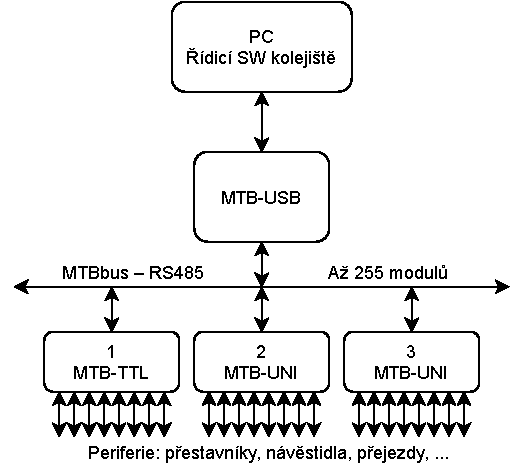
\includegraphics[width=0.7\textwidth]{data/mtb-topology.pdf}
\caption{Topologie systému \gls{mtb}.}
\label{fig:mtbbus-topology}
\end{figure}

\begin{table}[h]
	\begin{tabularx}{\textwidth}{XX}
		\toprule
		Typ přenosu & RS485, formát dat UART \\
		Komunikační rychlost & 38400~Bd, 57600~Bd, 115200~Bd \\
		Maximální počet modulů & 255 \\
		Počet datových bitů & 9 \\
		Stop bit & 1 \\
		Parita & žádná \\
		Maximální délka vedení & 100 m \\
		\bottomrule
	\end{tabularx}
	\caption{Základní parametry sběrnice \gls{mtbbus}}
	\label{tab:mtbbus-params}
\end{table}

Současná implementace sběrnice je založena na elektrickém standardu RS485.
Sběrnice RS485 je dvouvodičová (\textit{R+, R-, GND}) poloduplexní
diferenciální komunikační sběrnice vyvinutá s důrazem na odolnost vůči
externímu rušení. Je vhodná pro přenos dat na větší vzdálenosti, řádově desítky
až stovky metrů. Pro dosažení nejlepších elektrických vlastností by sběrnice
měla být lineární. Sběrnice je na obou koncích termínována rezistorem
\textit{200 R} a pull-up a pull-down rezistory pro držení definované úrovně
signálu.

Sběrnice RS485 je velice snadno implementovatelná do prakticky všech
mikrokontrolérů – stačí rozhraní UART, jeden pin pro řízení směru komunikace
a driver k RS485.

Na sběrnici mohou být \gls{mtb} moduly různého typu:

\begin{itemize}
\item \textbf{MTB-UNI}

	MTB-UNI (\textit{univerzální}) je nejpoužívanější typ modulu. Obsahuje 16
	digitálních vstupů a 16 digitálních výstupů. Na výstupech 0–7 umožňuje kódovat
	návěst protokolem S-COM \cite{}, což umožňuje připojení až 8 návěstidel
	k jednomu modulu MTB-UNI. Modul dále umožňuje připojení IR čidel na vstupy,
	což jsou rozšířená bodová čidla detekující průjezd vlaku. Pro použití IR
	čidel je třeba speciálním způsobem budit vysílací IR diodu, což si žádá podporu
	ve speciálním hardwaru na desce. Výstupu modulu jsou v režimu otevřeného
	kolektoru a umožňují maximální zátěž až 0.5~A / 8 výstupů.

\item \textbf{MTB-TTL}

	MTB-TTL je zjednodušený modul MTB-UNI. Oproti modulu MTB-UNI neobsahuje
	podporu IR čidel a výstupy má v režimu TTL. Od tohoto typu modulu se v
	současnosti ustupuje, neboť TTL výstupy nejsou vhodné pro spínání vyšších
	napětí (např. 12~V) a proto, že v případě neaktivního výstupu (+5~V –
	inverzní logika) aktivně napájí výstupní port, což způsobuje nechtěné chování,
	pokud je ne výstupním portu záměrně vypnutá periferie. V krajním případě může
	dojít až k přetížení TTL výstupu a jeho zničení. Na všechny nasazené moduly
	typu MTB-TTL byly postupně instalovány dodatečné obvody s otevřenými
	kolektory na výstupy.

\item \textbf{MTB-REG}

	MTB-REG je modul umožňující generovat analogový výkonový výstup. Modul se
	připojí ke kolejím a řídí rychlost a směr lokomotiv v řízeném úseku.

	Tento způsob řízení jízdy (tzv. \textit{analogový}) je dnes již překonaný.
	V současnosti se pro řízení jízdy lokomotiv na kolejišti používá tzv. systém
	\textit{Digital Command Control} \cite{dcc}, kde každá lokomtiva a mnohdy
	i vagóny v sobě mají mikroprocesor a celý systém je řízen digitálně.

	Modul MTB-REG je tedy již překonaným modulem a autor jej uvádí spíš pro
	úplnost popisu systému \gls{mtb}.

\item \textbf{MTB-POT}

	Modul MTB-POT obsahuje 4 analogové vstupy a 4 digitální vstupy. Jeho
	původním záměrem bylo, že se připojí k potenciometru v pultu obsluhy
	kolejiště, kterým obsluha reguluje jízdu vlaku. Po sběrnici přepošle data
	modulu \textit{MTB-REG} a tím dojde ke kýžené jízdě vlaku. Tento způsob
	řízení jízdy na kolejištích se již nepoužívá, proto i modul \textit{MTB-POT}
	pozbyl svého smyslu.

\end{itemize}

\begin{figure}[ht]
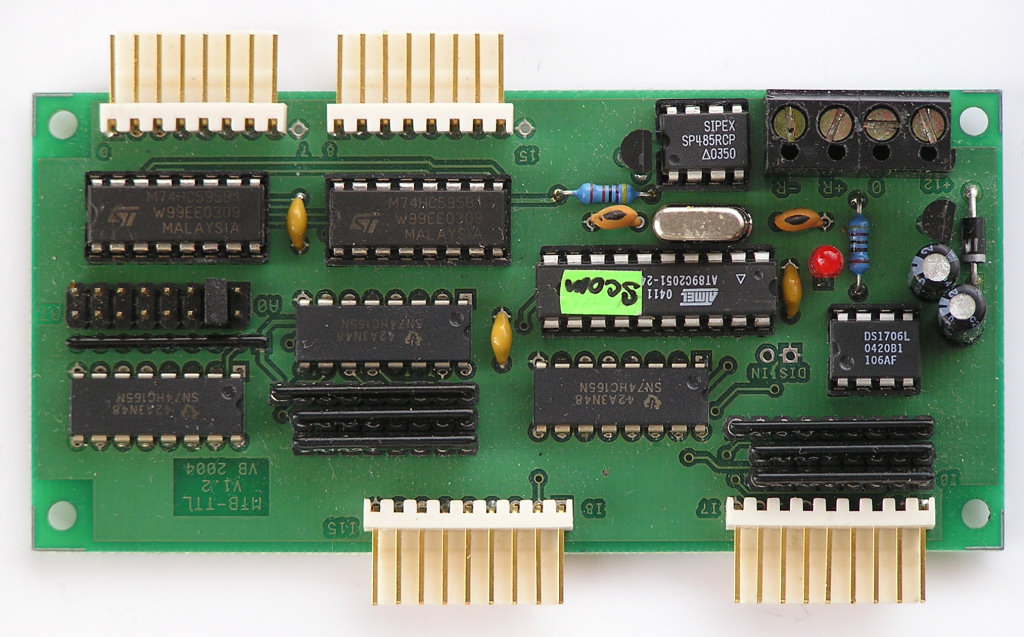
\includegraphics[width=0.7\textwidth]{data/mtbttl_foto.jpg}
\caption{Ukázka modulu MTB-TTL \cite{mtb:web}.}
\label{fig:mtbttl}
\end{figure}

Po sběrnici se komunikuje definovaným protokolem \cite{mtbbus-proto}. Protokol
definuje příkazy pro moduly, odpovědi modulů, časování apod.

Práce se sběrnicí z pohledu aplikace v počítači probíhá následovně:

\begin{compactenum}
\item Připojit se k MTB-USB modulu.
\item Provést sken aktivních modulů sběrnice.
\item Nahrát do všech aktivních modulů konfiguraci.
\item Přečíst stav vstupů.
\item Zahájit provoz – od teď všechny moduly nahlašují změnu stavu vstupu.
\item Číst vstupy, nastavovat výstupy.
\item Ukončit komunikaci.
\item Uzavřít spojení s MTB-USB.
\end{compactenum}

\section{Systém \gls{mtb} v kontextu řízení celého kolejiště} \label{sec:mtb_context}

V \gls{kmz} je aktuálně systém \gls{mtb} nasazen na dvou kolejištích, další
nasazení je na modulovém kolejišti Mendelovy univerzity v Brně, s kterou klub
spolupracuje. Na těch kolejištích je aktuálně nasazeno 99 MTB desek.

Pro zajímavost uveďme, jak systém MTB zapadá do celkové koncepce řízení
kolejiště.

\begin{figure}[ht]
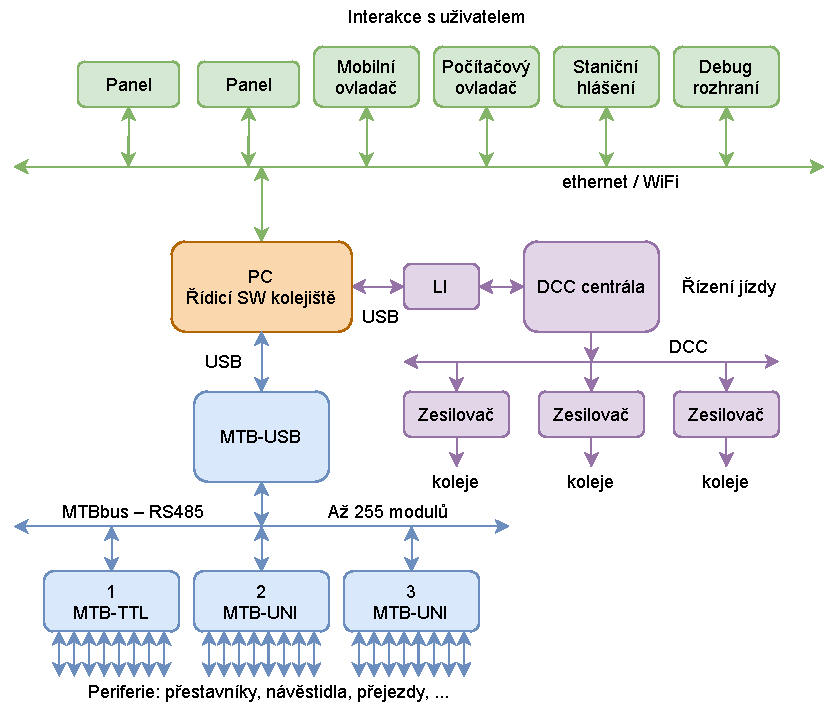
\includegraphics[width=\textwidth]{data/railroad-topology.pdf}
\caption{Schéma komponent řízení kolejiště v \gls{kmz}.}
\label{fig:railroad-topology}
\end{figure}
